\chapter{Introduction}

\section{Introduction}

ngscopeclient is a high performance, GPU accelerated remote user interface, signal processing, protocol analysis, and
automation tool for test and measurement equipment. It runs on all major operating systems and can interoperate with a
broad and continuously growing range of T\&M products from many vendors.

As of this writing, ngscopeclient is under active development but has not had a formal v0.1
release and should be considered alpha quality.

This is free software: you are free to change and redistribute it.
There is NO WARRANTY, to the extent permitted by law.

\section{Key Concepts}

\subsection{User Interface}

Most UI elements can be interacted with by left clicking (select), left dragging (move), using the scroll wheel (zoom),
double clicking (open properties dialog), or right clicking (context menu). Hovering the mouse over a main window UI
element, or a (?) help marker in a dialog box, displays a tooltip explaining the purpose of the element

%If you have a multi-button gaming mouse, button 8 stops the trigger and button 9 starts. These bindings are not
%currently configurable.

Most text fields allow SI prefixes for scaling values (mV, $\mu s$, GHz, etc). Lowercase `u' is interpreted as
``micro", equivalent to the Greek letter $\mu$. The unit is automatically added if not specified, for example typing
``2.4G" in a frequency input field will be interpreted as meaning 2.4 GHz.

\subsection{Design Philosophy}

Users familiar with conventional benchtop oscilloscopes will notice some important distinctions between ngscopeclient
and classical DSO user interfaces. While there is an initial learning curve getting used to the different ways of doing
things, these changes allow for greater productivity and more complex analysis.

Legacy DSO user interfaces largely still imitate the front panel controls of analog CRT instruments dating back to the
mid 1940s. A single view of each waveform shows the entire acquisition on a grid with a fixed number of divisions
(emulating an etched graticule on a CRT) and both time and voltage scales are defined in terms of these divisions.
While more recent DSOs do allow math functions, protocol decodes, zooms, and so on, this archaic concept has remained.

In ngscopeclient, the acquisition record length is completely decoupled from the X axis scale of the viewport, and
there is no concept of a ``zoom" waveform or measuring time in ``divisions". Arbitrarily many views of a channel may be
created, and each may be scaled and zoomed independently. Acquisition record length and duration are controlled
separately, from the timebase properties dialog.

Similarly, vertical scale for waveforms is defined in terms of full-scale range, a far more intuitive and useful metric
than arbitrary ``divisions". While horizontal grid lines are still displayed in waveform views for convenience, their
number, spacing, and locations may change. Tall plots will have more scale divisions than short ones, and the divisions
are always located at round numbers even if this requires the grid to not be centered in the plot (Fig. \ref{y-divs})

\begin{figure}[h]
\centering
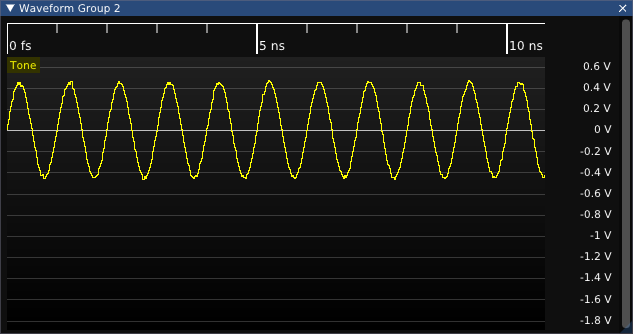
\includegraphics[width=13cm]{ng-images/y-divs.png}
\caption{Example waveform showing off-center grid and round-numbered grid lines}
\label{y-divs}
\end{figure}

Rather than optimizing for a touch screen (as is common for benchtop oscilloscopes), ngscopeclient's UI is
heavily mouse driven and context based. Space used by always-visible buttons, sliders, etc is kept to a minimum in
order to keep as much screen real estate as possible usable for waveform display. Additional controls are displayed in
menus or pop-up dialogs which can be closed, moved out of view, or docked as needed.

\subsection{Terminology}

The overall software package consists of \emph{ngscopeclient} (graphical user interface frontend), \emph{libscopehal}
(C++ library for core APIs and instrument drivers), and \emph{libscopeprotocols} (filter graph blocks). End users will
normally use ngscopeclient, however it is possible to interface with libscopehal and libscopeprotocols directly from
C++ code for writing low level test automation tools or even a fully custom application-specific user interface.

Data consists of two fundamental types: \emph{scalars} and \emph{waveforms}. A scalar is a single numeric value with an
associated unit, for example ``500 mV". A waveform is a sequence of \emph{samples} plotted against another quantity, for
example voltage versus time for an oscilloscope waveform or amplitude versus frequency for a spectrum analyzer
waveform.

Samples may be of arbitrary type (analog value, digital bit, SPI bus event, etc.), but all samples in a
single waveform must be of the same data type. Waveforms may be either \emph{uniform} (sampled at constant rate with no
gaps between samples) or \emph{sparse} (sampled at arbitrary intervals, possibly with gaps between samples).

An \emph{instrument} is a physical piece of hardware \footnote{Or a simulated mock-up of one, such as the ``demo"
oscilloscope driver used for testing} which can be remote controlled and interacted with. The connection between
ngscopeclient and an instrument is provided by a \emph{transport}, such as a USBTMC interface, a GPIB data stream, or a
TCP socket. A \emph{driver} is a software component, either supplied as part of the libscopehal core or a third party
plugin, which controls an instrument.

Each instrument has one or more\footnote{Zero channels is legal in the API, however such an instrument would be of
little practical use!} \emph{channels}. A channel corresponds to a single logical ``piece" of an instrument and may
consist of one or more physical connectors: a typical oscilloscope channel has a single BNC input while a typical power
supply output has two banana jacks.

Each channel may provide features associated with one or more instrument \emph{types}, and not all channels on an
instrument are guaranteed to be the same type(s). For example, an oscilloscope may consist of several channels
providing both waveform acquisition (oscilloscope) and scalar acquisition (multimeter) capabilities, one channel
providing only trigger input capability, and one channel providing function generator output capability.

All channels, triggers, and math / protocol decode blocks are considered \emph{nodes} within the \emph{filter graph}.
The filter graph is a directed acyclic graph (a set of nodes and connections between them, with no loops permitted)
connecting all of the various data inputs and outputs of the experimental setup together.

Each node may have zero or more \emph{inputs}, of either scalar or waveform type, and zero or more output
\emph{streams}. A stream is a data source which may or may not have an associated scalar or waveform value; for example
a math block with missing inputs or an instrument which has not yet triggered do not have a meaningful value. A typical
oscilloscope channel might have one waveform output stream, while a typical power supply channel might have two scalar
output streams for measured current and voltage. A sink block for writing a waveform to a CSV file would have one input
for each column in the generated file.

Instrument hardware limitations or the particular math/decode block's design will impose various restrictions on legal
connections in the filter graph. For example, a trigger can normally only accept signals from hardware input channels
on the same instrument. An FFT filter can only accept uniformly sampled analog waveforms. A UART protocol decode can
only accept digital waveforms, so analog waveforms must be converted to digital by a thresholding filter before they
can be decoded.

\section{Revision History}
\begin{itemize}
\item \today: [in progress] Initial draft
\end{itemize}
